\section{Recursive Bayesian Parameter Estimation}
In this section, we provide a theoretical background to recursive bayesian parameter estimation as a complement to our last contribution.
In particular, this contribution relies on estimating class-priors on every frame of a sequence, i.e. estimating the proportion of positive over-segmented regions.

Here, we start by formulating the state-estimation problem using the hidden Markov model framework.
Next, we show how the traditional Kalman filtering algorithm \cite{kalman1960} allows to estimate a posteriori state-estimates using observations in an efficient manner when specific assumptions are validated.
We then elaborate on the \gls{ekf} and its successor, the \gls{ukf}

\subsection{Hidden Markov model}
In recursive bayesian parameter estimation, we aim at estimating the true value of a state variable $\bm{x}$ over time, by leveraging incoming noisy observations $\bm{z}$.
We assume that a mathematical model exists that evolve the current true value of the state to the state at the previous time-step.
Furthermore, another model provides the relation between the observation of and the state.
Formally, we define the following discrete-time dynamic system:

\begin{align}
  \bm{x}_{k+1}&=F(\bm{x}_{k},\bm{v}_{k}) \label{eq:bg_state_trans}\\
  \bm{z}_{k}&= H(\bm{x}_{k}, \bm{n}_{k}) \label{eq:bg_proc}
\end{align}

where $\bm{x}$ denotes the state variable, $\bm{z}$ denotes the observations,
$F$ and $H$ are the transition and process models, respectively, while $\bm{v}$ and $\bm{n}$ are the process and transition noise, respectively.
Fig. \ref{fig:hmm} represents the dynamic system of Eq. \ref{eq:bg_state_trans} and \ref{eq:bg_proc} as a directed graph, where edges represent probabilistic relationships.
In the recursive bayesian filtering paradigm, we assume that all variables are stochastic.
Furthermore, the systems follows the Markov assumption, i.e. every variable is conditionally independent of its non-descendants, given its parents \cite{geiger90}.
Formally,

\begin{align}
  p(\bm{x}_{k+1}|\bm{x}_{k}, \bm{x}_{k-1},\ldots,\bm{x}_{0})=p(\bm{x}_{k+1}|\bm{x}_{k})\\
  p(\bm{z}_{k}|\bm{x}_{k}, \bm{x}_{k-1},\ldots,\bm{x}_{0})=p(\bm{z}_{k}|\bm{x}_{k})
\end{align}

When the state variables are unobserved, but is dependent on another observable process, we call such a system a \gls{hmm}.

\begin{figure}[!htpb]
  \centering
  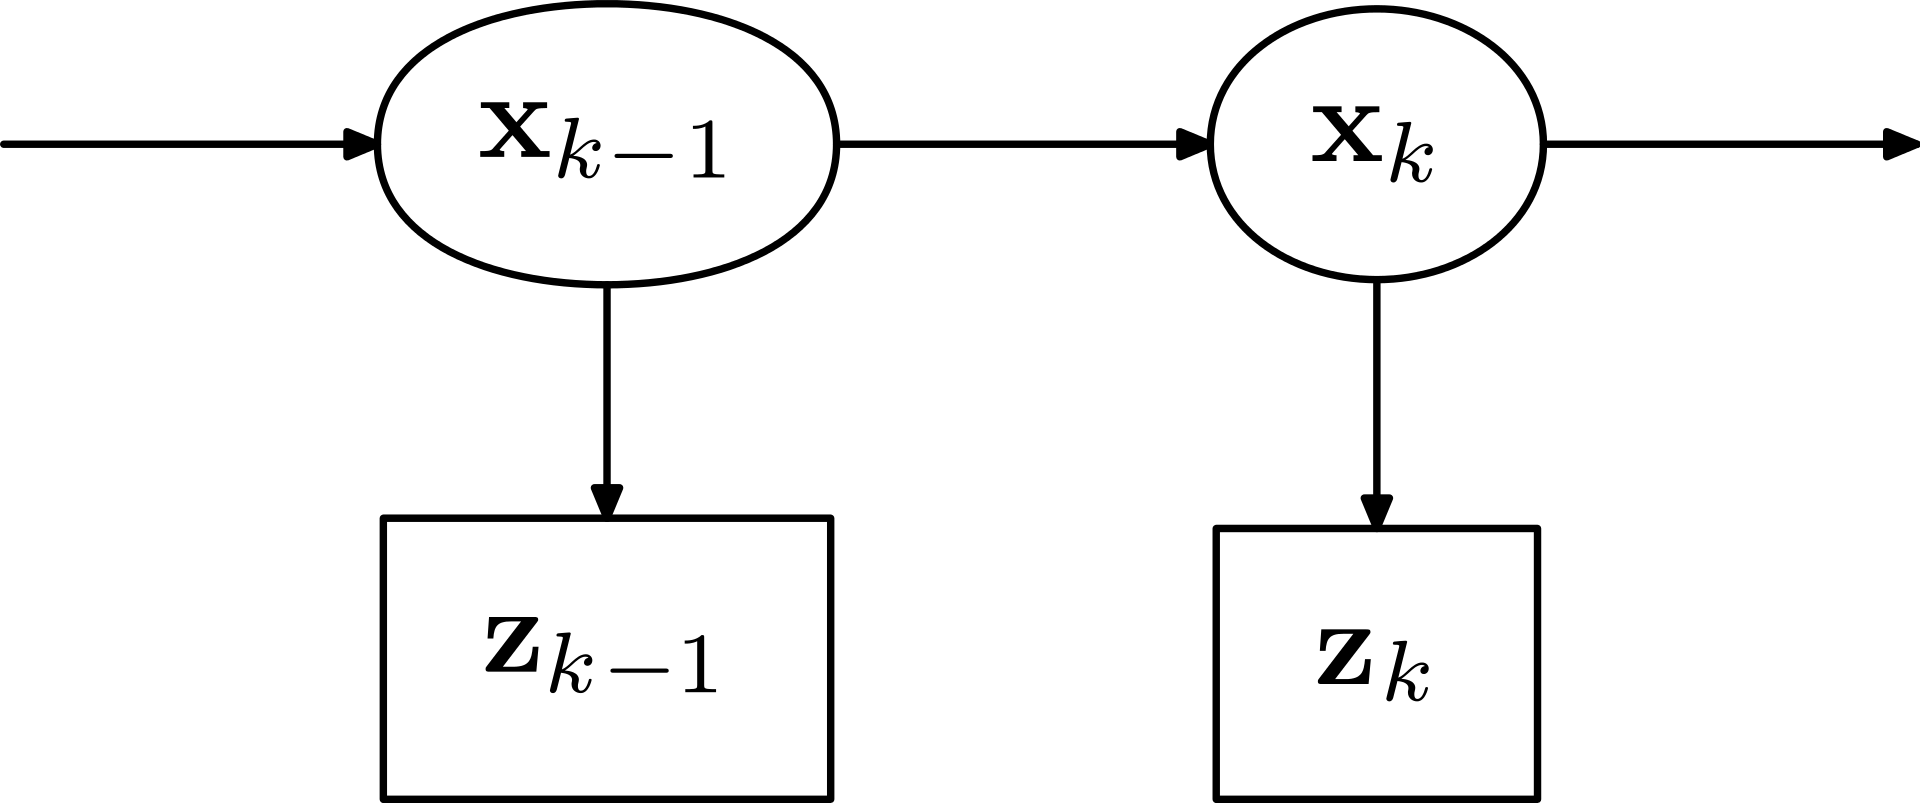
\includegraphics[width=10cm]{hmm}
  \caption{Graphical representation of a \gls{hmm}. $x$ are the hidden variables, while $z$ are the observations.
  Edges represent probabilistic relationships.}
  \label{fig:hmm}
\end{figure}

\subsection{Recursive bayesian filtering and Kalman Filter Equations}
In recursive bayesian filtering, we are interested in estimating the \gls{pdf} of the current state using the history of observations up to the current time-step, written $p(\bm{x}_{k}|\bm{z}_{0:k}$, where $\bm{z}_{0:k}$ is a short form for $\bm{z}_{0},\ldots, \bm{z}_{k}$.

Using Baye's rule, we rewrite:
\begin{equation}
  \label{eq:bg_aposteriori}
  p(\bm{x}_{k}|\bm{z}_{0:k}) = \frac{p(\bm{x}_{k}|\bm{z}_{0:k-1})\cdot p(\bm{x}_{k}|\bm{z}_{k})}{p(\bm{x}_{k}|\bm{z}_{0:k-1})}
\end{equation}

The left term of the denominator of Eq. \ref{eq:bg_aposteriori} is called the a-priori probability distribution of the current state.
We rewrite it in a recursive form as
\begin{equation}
  \label{eq:bg_prior}
  p(\bm{x}_{k}|\bm{z}_{0:k-1}) = \int p(\bm{x}_{k}|\bm{x}_{k-1}) \cdot p(\bm{x}_{k-1}|\bm{z}_{0:k-1}) d\bm{x}_{k-1}
\end{equation}

Next, the denominator is a normalization term written:
\begin{equation}
  \label{eq:bg_norm_cst}
  p(\bm{z}_{k}|\bm{z}_{0:k-1}) = \int p(\bm{x}_{k}|\bm{z}_{0:k-1}) \cdot p(\bm{z}_{k}|\bm{x}_{k}) d\bm{x}_{k}
\end{equation}

In this general form, the exact inference of Eq. \ref{eq:bg_aposteriori} is untracktable.
However, many algorithms exists that solve this problems approximately under specific conditions, e.g. Expectation-Maximization \cite{dempster77} and Markov-chain Monte Carlo \cite{geyer92}.

\subsubsection{Kalman Filter}

Under the more restrictive assumptions that (1) models $F$ and $G$ are linear functions, (2) the initial values of the state variables follow a multivariate normal distribution, and (3) the process and observation noise are additive, zero-mean and normally distributed, the \gls{kf} algorithm provides exact solutions.
This comes from the fact that under the above conditions, the a-posteriori pdf \ref{eq:bg_aposteriori} is also normally distributed, and is therefore fully characterized by its first and second moment, i.e. its mean and covariance.
Under these conditions, the condition \gls{pdf} is fully characterized by its first and second moment, i.e. mean and covariance.

the \gls{kf} only needs to propagate the
Under these assumptions, the state-space model is rewritten :

\begin{align}
  \bm{x}_{k+1}&=F_{k}\bm{x}_{k} B_{k}u_{k} + \bm{v}_{k} \label{eq:bg_state_trans_kf}\\
  \bm{z}_{k}&= H_{k}\bm{x}_{k} + \bm{n}_{k} \label{eq:bg_proc_kf} \\
  \bm{x}_{0}&= \bm{\bar{x}}_{0} + \mathcal{N}(0,S) \label{eq:bg_init_kf}
\end{align}

Where $\bm{v}_{k}=\mathcal{N}(0,Q)$, $\bm{n}_{k}=\mathcal{N}(0,R)$ are the process and observation noise signals, respectively, while $Q$, $R$, and $S$ are the process, observation and initial covariance matrices, respectively.

\subsubsection{Kalman Filter inference}
We now provide an overview of the main steps of the \gls{kf} algorithm.
For the detailed derivations, we refer the reader to \cite{thacker98}.

The problem of \gls{kf} is to produce an optimal estimate of the hidden state variable, written $\bm{\hat x}_{k}$, given the observations.
In particular, it takes as criteria of optimality the \gls{mse} between the estimate and the true value of the state.
As shown in \cite{ribeiro04}, the estimator that minimizes this criteria is the the conditional mean, i.e.

\begin{equation}
  \label{eq:bg_cond_mean}
  \bm{\hat x}_{k} = \mathbb{E}[\bm{x}_{k}|\bm{z}_{0:k}]
\end{equation}

The inference is decomposed into a prediction and filtering step, i.e.

\begin{itemize}
    \item \textbf{Prediction: } $p(\bm{x}_{k}|\bm{z}_{0:k}) \rightarrow p(\bm{x}_{k+1}|\bm{z}_{0:k})$
    \item \textbf{filtering: } $p(\bm{x}_{k+1}|\bm{z}_{0:k}) \rightarrow p(\bm{x}_{k+1}|\bm{z}_{0:k+1})$
\end{itemize}

Where the prediction step applies the transition function to the current state estimate, thereby computing the a-priori conditional \gls{pdf}, and the filtering corrects the latter using the newly arrived observation $\bm{z}_{k+1}$, thereby computing the a-posteriori conditional \gls{pdf}.

Formally, the prediction step resolves to the following recursive equation:

\textbf{Prediction:}
\begin{align}
  \bm{\hat x}^{-}_{k+1}&=F_{k} \bm{\hat x}_{k} + B_{k}u_{k} \label{eq:bg_apriori_estim}\\
  P_{k+1}^{-}&=F_{k} P_{k} F_{k}^{T} + Q_{k} \label{eq:bg_apriori_cov}
\end{align}

Where $P_{k}$ is the covariance matrix of the state, and $\bm{\hat x}^{-}$ denotes the a-priori state estimate.
Eq. \ref{eq:bg_apriori_estim} computes the a-priori state estimate, and Eq. \ref{eq:bg_apriori_cov} computes the a-priori state covariance.

\textbf{Correction:}
\begin{align}
  \bm{\tilde y}_{k+1} &= \bm{z}_{k+1} - H_{k+1} \bm{\hat x}_{k+1}^{-} \label{eq:bg_innov} \\
  T_{k+1} &= H_{k+1} P_{k+1}^{-} H_{k+1}^{T} + R_{k} \label{eq:bg_innov_cov} \\
  K_{k+1} &= P_{k+1}^{-} H_{k+1}^{T} T_{k+1}^{T} \label{eq:bg_kf_gain}\\
  \bm{\hat x}_{k+1} &= \bm{\hat x}_{k+1} + K_{k} \bm{\tilde y}_{k+1} \label{eq:bg_aposteriori_state_estim}\\
  P_{k+1} &= (I - K_{k+1}H_{k+1}) P_{k+1}^{-} \label{eq:bg_aposteriori_cov_estim}
\end{align}

Eq. \cref{eq:bg_innov,eq:bg_innov_cov,eq:bg_kf_gain,eq:bg_aposteriori_state_estim,eq:bg_aposteriori_cov_estim} compute the state innovation, covariance innovation, Kalman gain, a-posteriori state estimate, and a-posteriori covariance estimate, respectively.
In practice, the two above steps are applied each time a new observation arrives.

\subsection{Unscented Kalman Filter}
The standard \gls{kf} framework allows to compute the a-priori state estimate, Kalman gain, and a-posteriori state estimate \textit{exactly}, by propagating the mean and covariance of the state, two quantities that fully characterize its \gls{pdf}, through the linear-system dynamics.
However, when the system is non-linear, the \gls{kf} is prohibited, since the a-priori and a-posteriori conditional \gls{pdf}, after transformation, become non-gaussian.
The \gls{ekf} \cite{ribeiro04} attempts to generalize \gls{kf} to such scenario by approximating the moments of these \gls{pdf} using first-order Taylor expansion around the current estimates.
We choose not to delve into the details of \gls{ekf}, and simply mention that the latter approximation, in practice, bring sub-optimal results and often lead to the divergence of the filter \cite{wan00}.

We now give an overview of the \gls{ukf}, which attempts to amend the flaws of \gls{ekf}.

\subsubsection{Unscented Transformation}
\gls{ukf} considers the \gls{ut} \cite{julier96}, which discretize a (continuous) \gls{pdf} into a set of carefully chosen points so as to (1) capture the true mean and covariance accurately, and (2) capture the true posterior statistics up to the third order after propagation through non-linear functions.
This approach departs from \gls{ekf} in that, the non-linear functions are applied to these transformed points directly.

In particular, let $\bm{x}$ a \gls{grv} of dimension $L$ with mean $\bm{\bar x}$ and covariance $P_{x} \in \mathbb{R}^{L \cdot L}$.
The goal is to find a set of $2L$ from the rows or columns of the matrices $\pm \sqrt{L P_{x}}$ with zero mean and sample covariance $P$, and apply a translation of each point to get a mean of $\bm{\bar x}$.
We let $\bm{\mathcal{X}}$ a matrix whose rows contain $2L+1$ sigma-vectors $\bm{\mathcal{X}}_{i}$, and $\mathcal{Y} = g(\mathcal{X})$ its transformation trough an arbitrary function $g$.
The procedure is \cite{wan00}:
\begin{enumerate}
  \item Compute sigma-points $\mathcal{X}$ and corresponding weight matrix $W$ as:
    \begin{itemize}
      \item $\mathcal{\bm{X}}_{0} = \bm{\bar x}$
      \item $\mathcal{\bm{X}}_{i} = \bm{\bar x} + (\sqrt{(L + \lambda) P_{x}})_{i} \quad i=1,\ldots,L$
      \item $\mathcal{\bm{X}}_{i} = \bm{\bar x} - (\sqrt{(L + \lambda) P_{x}})_{i} \quad i=L+1,\ldots,2L+1$
      \item $W_{0}^{(m)}=\lambda / (L + \lambda)$
      \item $W_{0}^{(c)}=\lambda / (L + \lambda) + (3 - \alpha^{2})$
      \item $W_{i}^{(m)}=W_{i}^{(c)}= 1 / [2(L + \lambda)]$
    \end{itemize}
\end{enumerate}

Where $\lambda = L (\alpha^{2}-1)$ is a scaling parameter, and $\alpha$ determines the spread of sigma points around the mean.
Next, the sigma-points are propagated through $g$:
\begin{equation}
  \mathcal{Y}_{i} = g(\mathcal{X}_{i}) \quad i=0,\ldots,L
\end{equation}
Finally, we obtain the statistics of the output through the following approximations:
\begin{align}
  \bm{\bar y} & \approx \sum_{i=0}^{2L} W_{i}^{(m)}\mathcal{Y}_{i} \\
  P_{y} & \approx \sum_{i=0}^{2L} W_{i}^{(c)}[\mathcal{Y}_{i}-\bm{\bar y}][\mathcal{Y}_{i}-\bm{\bar y}]^{T}
\end{align}

\begin{figure}[!htpb]
  \centering
  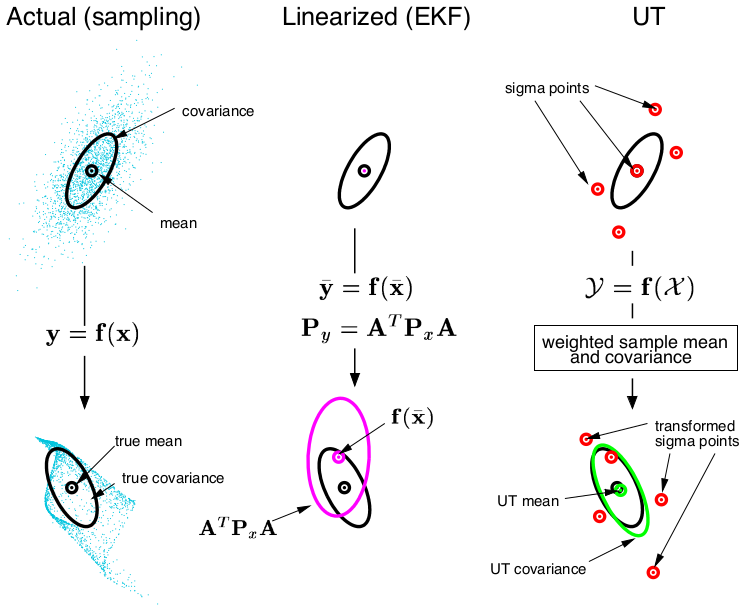
\includegraphics[width=10cm]{ukf}
  \caption{Example of the Unscented Transformation and its mean and covariance after the propagation step.
  (a) Monte Carlo sampling (b) Extended Kalman Filter (linearized) (c) Unscented Transformation (UKF). Taken from \cite{wan00}.}
  \label{fig:ukf}
\end{figure}

Fig. \ref{fig:ukf} illustrates three strategies where a \gls{pdf} is propagated through a non-linear function, where the first samples arbitrary points, the second performs a linearization of the function as in \gls{ekf}, and the third follows the above \gls{ut} strategy.

The full procedure for \gls{ukf} is identical to the original \gls{kf}, i.e. performs
a prediction step (as in \cref{eq:bg_apriori_estim,eq:bg_apriori_cov}), and
a correction step (as in \cref{eq:bg_innov,eq:bg_innov_cov,eq:bg_kf_gain,eq:bg_aposteriori_state_estim,eq:bg_aposteriori_cov_estim}) by applying the above sigma-points sampling and propagation step.

%%% Local Variables:
%%% mode: latex
%%% TeX-master: "../../main"
%%% End:
